\documentclass[10pt]{beamer}\usepackage[]{graphicx}\usepackage[]{color}
%% maxwidth is the original width if it is less than linewidth
%% otherwise use linewidth (to make sure the graphics do not exceed the margin)
\makeatletter
\def\maxwidth{ %
  \ifdim\Gin@nat@width>\linewidth
    \linewidth
  \else
    \Gin@nat@width
  \fi
}
\makeatother

\definecolor{fgcolor}{rgb}{0.345, 0.345, 0.345}
\newcommand{\hlnum}[1]{\textcolor[rgb]{0.686,0.059,0.569}{#1}}%
\newcommand{\hlstr}[1]{\textcolor[rgb]{0.192,0.494,0.8}{#1}}%
\newcommand{\hlcom}[1]{\textcolor[rgb]{0.678,0.584,0.686}{\textit{#1}}}%
\newcommand{\hlopt}[1]{\textcolor[rgb]{0,0,0}{#1}}%
\newcommand{\hlstd}[1]{\textcolor[rgb]{0.345,0.345,0.345}{#1}}%
\newcommand{\hlkwa}[1]{\textcolor[rgb]{0.161,0.373,0.58}{\textbf{#1}}}%
\newcommand{\hlkwb}[1]{\textcolor[rgb]{0.69,0.353,0.396}{#1}}%
\newcommand{\hlkwc}[1]{\textcolor[rgb]{0.333,0.667,0.333}{#1}}%
\newcommand{\hlkwd}[1]{\textcolor[rgb]{0.737,0.353,0.396}{\textbf{#1}}}%

\usepackage{framed}
\makeatletter
\newenvironment{kframe}{%
 \def\at@end@of@kframe{}%
 \ifinner\ifhmode%
  \def\at@end@of@kframe{\end{minipage}}%
  \begin{minipage}{\columnwidth}%
 \fi\fi%
 \def\FrameCommand##1{\hskip\@totalleftmargin \hskip-\fboxsep
 \colorbox{shadecolor}{##1}\hskip-\fboxsep
     % There is no \\@totalrightmargin, so:
     \hskip-\linewidth \hskip-\@totalleftmargin \hskip\columnwidth}%
 \MakeFramed {\advance\hsize-\width
   \@totalleftmargin\z@ \linewidth\hsize
   \@setminipage}}%
 {\par\unskip\endMakeFramed%
 \at@end@of@kframe}
\makeatother

\definecolor{shadecolor}{rgb}{.97, .97, .97}
\definecolor{messagecolor}{rgb}{0, 0, 0}
\definecolor{warningcolor}{rgb}{1, 0, 1}
\definecolor{errorcolor}{rgb}{1, 0, 0}
\newenvironment{knitrout}{}{} % an empty environment to be redefined in TeX

\usepackage{alltt}
\usepackage{etex}

\usepackage[T1]{fontenc}
\usepackage{textpos} 
\usepackage{hyperref}
\usepackage{amsmath,amsthm,amsfonts,nicefrac,mathabx,amssymb,amsbsy}
 \usepackage[subnum]{cases}
\usepackage{calligra, mathrsfs}
%\usepackage{natbib}
\usepackage{booktabs}
%\bibpunct{(}{)}{;}{a}{,}{,}
\usepackage[english]{babel}
\usepackage[latin1]{inputenc}
\usepackage{helvet}
\usepackage{graphicx}
\usepackage{color}
\usepackage{multirow,dcolumn}
\usepackage{listings}
\usepackage{ragged2e}
\usepackage{xcolor}
\usepackage{colortbl}
\usepackage{booktabs}
\usepackage{enumitem}
\usepackage{animate} %for animated graphs
\usepackage{graphicx}
\usepackage{tikz}
\usetikzlibrary{calc}
\usepackage{url}
\usepackage{bibentry}
\usepackage{chngcntr}

\ifx\hypersetup\undefined
  \AtBeginDocument{%
    \hypersetup{unicode=true,pdfusetitle,
 bookmarks=true,bookmarksnumbered=false,bookmarksopen=false,
 breaklinks=false,pdfborder={0 0 0},backref=false,colorlinks=false}
  }
\else
  \hypersetup{unicode=true,pdfusetitle,
 bookmarks=true,bookmarksnumbered=false,bookmarksopen=false,
 breaklinks=false,pdfborder={0 0 0},backref=false,colorlinks=false}
\fi

\colorlet{tablesubheadcolor}{gray!25}
\colorlet{tableheadcolor}{gray!40}
\colorlet{tablerowcolor}{gray!15.0}
\usetheme{Gesis}
%\setbeamertemplate{navigation symbols}{}
\setbeamertemplate{footline}[frame number]%{\hspace*{.2cm}\insertframenumber}
\setbeamerfont{caption}{size=\footnotesize}
\usefonttheme[onlylarge]{structuresmallcapsserif} % alte Schrift


\definecolor{hellgrau}{rgb}   {0.109375,  0.40625,   0.51953125}
\definecolor{dunkelgrau}{rgb} {0.009375,  0.30625,   0.41953125}
\definecolor{dunkelgrau2}{rgb}{0.009375,  0.20625,   0.31953125}
\definecolor{hellbraun}{rgb}  {0.9140625, 0.8984375, 0.8046875}
\definecolor{hellbraun2}{rgb} {.95,       0.9,       0.8}
\definecolor{alertred}{rgb}   {0.8515625, 0.3828125, 0.08984375}
\definecolor{orange}{rgb}{1,0.5,0}


\setbeamercolor{firstsecslide}{fg=white,bg=dunkelgrau}
\setbeamertemplate{blocks}[rounded][shadow=true]

\newcolumntype{d}[1]{D{.}{.}{#1}}

\newcommand{\emphred}[1]{\textcolor{alertred}{#1}}
\newcommand{\emphcol}[1]{\textcolor{dunkelgrau}{\slshape #1}}

\newcommand{\eqname}[1]{\tag*{#1}} %equation title

\newenvironment{frcseries}{\fontfamily{frc}\selectfont}{}
\newcommand{\textfrc}[1]{{\frcseries#1}}
\newcommand{\mathfrc}[1]{\text{\textfrc{#1}}}


\setcounter{tocdepth}{1}
\setbeamercolor*{section in toc}{fg=hellgrau}
\setbeamertemplate{bibliography item}[default]


\setcounter{secnumdepth}{3}
\setcounter{tocdepth}{3}

\newsavebox{\mysavebox}


\newcommand{\E}[1]{\text{E}\left(#1\right)}
\newcommand{\V}[1]{\text{V}\left(#1\right)}
\newcommand{\AV}[1]{\text{AV}\left(#1\right)}
\newcommand{\Vest}[1]{\widehat{\text{V}}\left(#1\right)}
\newcommand{\MSE}[1]{\text{MSE}\left(#1\right)}
\newcommand{\COV}[2]{\text{COV}\left(#1,\,#2\right)}
\newcommand{\deff}{\ensuremath{\text{\slshape deff}}}
%roman numbers in equation
\newcommand{\RN}[1]{%
  \textup{\uppercase\expandafter{\romannumeral#1}}%
}


\makeatletter

\addtobeamertemplate{frametitle}{}{%
\begin{textblock*}{100mm}(.91\textwidth,-1cm)

\includegraphics[height=1cm,width=2cm]{../common/pics/GESIS_Logo_kompakt_en.jpg}
\end{textblock*}}




%%%%%%%%%%%%%%%%%%%%%%%%%%%%%% LyX specific LaTeX commands.
\providecommand{\LyX}{\texorpdfstring%
  {L\kern-.1667em\lower.25em\hbox{Y}\kern-.125emX\@}
  {LyX}}

%%%%%%%%%%%%%%%%%%%%%%%%%%%%% Textclass specific LaTeX commands.
% this default might be overridden by plain title style
 \newcommand\makebeamertitle{\frame{\maketitle}}%
 % (ERT) argument for the TOC
 \AtBeginDocument{%
   \let\origtableofcontents=\tableofcontents
   \def\tableofcontents{\@ifnextchar[{\origtableofcontents}{\gobbletableofcontents}}
   \def\gobbletableofcontents#1{\origtableofcontents}
 }

%%%%%%%%%%%%%%%%%%%%%%%%%%%%%% User specified LaTeX commands.
%\usetheme{Montpellier}%\usetheme{PaloAlto}

\makeatother
\IfFileExists{upquote.sty}{\usepackage{upquote}}{}
\begin{document}



\title[Estimation]{Sampling and Estimation}   
\subtitle{Part 3: Calibration Weights}

\author{Stefan Zins\thanks{\href{mailto:Stefan.Zins@gesis.org}{Stefan.Zins@gesis.org}}, Matthias Sand\thanks{\href{mailto:Matthias.Sand@gesis.org}{Matthias.Sand@gesis.org}}, and Jan-Philipp Kolb\thanks{\href{mailto:Jan-Philipp.Kolb@gesis.org}{Jan-Philipp.Kolb@gesis.org}}}
\date{\today} 

\makebeamertitle

\begin{frame}[fragile]{Survey Imperfections}
\begin{figure}[H]
\begin{minipage}[c]{1\textwidth}
%            \label{Missings}
                \centering
%\noindent{\caption{\small{\textbf{Stichprobenziehung}}}}
\vspace{.25cm}
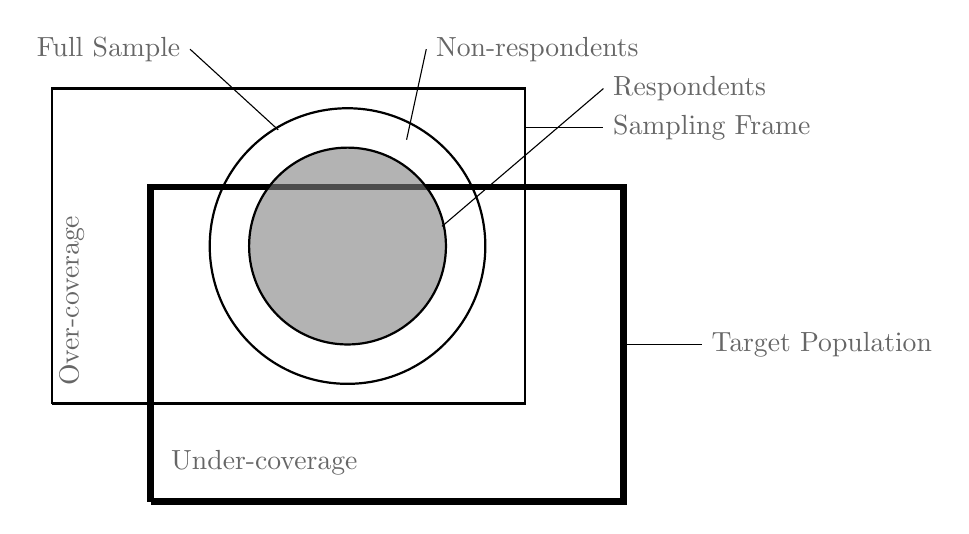
\begin{tikzpicture}[scale=1, fill opacity=0.6,font=\normalsize]
\draw[black,line width=2.5pt] (0,0) -- ++(0:6cm) -- ++(90:4cm) -- ++(180:6cm) -- ++(270:4cm);
\draw[black,thick] (-1.25,1.25) -- ++(0:6cm) -- ++(90:4cm) -- ++(180:6cm) -- ++(270:4cm);
\draw[ draw = black,thick] (2.5,3.25) circle (1.75);
\draw[fill=black!50, draw = black,thick] (2.5,3.25) circle (1.25);

\coordinate[label=right:Target Population] (A) at (7,2);
\draw (6,2) -- (A);
\coordinate[label=right:Sampling Frame] (B) at (5.75,4.75);
\draw (4.75,4.75) -- (B);
\coordinate[label=left:Full Sample] (C) at (0.5,5.75);
\draw (1.62,4.725) -- (C);
\coordinate[label=right:Non-respondents] (D) at (3.5,5.75);
\draw (3.25,4.6) -- (D);
\coordinate[label=right:Respondents] (E) at (5.75,5.25);
\draw (3.7,3.5) -- (E);
\coordinate[label=left:Under-coverage] (F) at (2.75,0.5);
\coordinate[label=above:\rotatebox{90}{Over-coverage}] (G) at (-1,1.35);
\end{tikzpicture}
%\centering\small{\textbf{Angaben in Prozent}}
\end{minipage}
\end{figure}
\end{frame}

% 
\frame{
  \frametitle{Methods to Handle Missing Data}

\begin{itemize}
 \item<1->  Procedures based on the {\bf available cases} only, i.e., only those cases that are completely
 recorded for the variables of interest.
 \item<2-|alert@5> {\bf Weighting procedures} that adjust design weights to compensate the bias that a MAR non-response might inflict on HT-type estimators.
 \item<3-> {\bf Single imputation} and correction of the variance estimates to
 account for imputation uncertainty.
 \item<4-> {\bf Multiple imputation} (MI).
%  \item {\bf Model-based corrections} of parameter estimates such as the
%  expectation-maximization (EM) algorithm
 \end{itemize}

\onslide+<5>{$\boldsymbol{\longrightarrow}$\quad {Methods for handling coverage errors are not so widely spread, simply because there is often no reliable auxiliary information on just the target population. However if there is, it can receive a treatment similar to that of weighting by non-response.}
}
}


\begin{frame}{Missing Data} 
\emph{Missing data is the norm, rather than the exception!}

%\begin{minipage}[h]{8cm}
% \begin{center}
Missingness may be either
\begin{description} 
  \item[MCAR]<2-> missing completely at random,  
   \begin{itemize}
     \item every unit has same response propensity (RP);
     \item respondents are a random sample of the initial sample
   \end{itemize}
  \item[MAR]<3->  missing at random, or
   \begin{itemize}
     \item RP depends on auxiliary variables $\boldsymbol{\mathcal{X}}$;
     \item can be modeled, if $\boldsymbol{\mathcal{X}}$ is known for both respondents \& non-respondents
   \end{itemize}
  \item[MNAR]<4-> missing not at random \vspace{2mm}
  \begin{itemize}
    \item RP depends on variables of interest $\mathcal{Y}$; 
    \item cannot be modeled, because $\mathcal{Y}$ not known for non-respondents
  \end{itemize}
\end{description}
\uncover<4>{ (see \cite{LittleRubin2002}) 
%\end{center}\vspace*{3mm}
%\end{minipage}
~\\[3mm]
$\boldsymbol{\longrightarrow}$\quad {In
multivariate analysis 30\% to 40\% of the data are often lost with
case deletion, assuming MCAR!}
}
\end{frame}



\section{Weighting Methods}

 \begin{frame}{Weighting Methods}

\begin{description}
\item[Calibration approach]<1|only@1> The design weighs are calibrated to the totals of some auxiliary variables $\boldsymbol{\mathcal{X}}$ (see  \cite{SaerndalLundstroem2005}).
\begin{itemize}
  \item Sample estimates using the calibrated weights will exactly replicated those totals.
  \item If the used auxiliary variables help to explain the response process the calibrated weight can reduce the non-response error.
\end{itemize}
\item[Two-phase approach]<2|only@2> The response process is modeled to obtain the response propensities $\psi_k$ for all $k \in \mathfrc{s}$. The new weight of element $k$ is $\frac{d_k}{\psi_k}$. (Two phases: 1. Sampling $\boldsymbol{\rightarrow}$ 2. Responding). 
\item<2|only@2> In addition the new weights $\frac{d_k}{\psi_k}$ might then also be calibrated. 
\item<2|only@2> Often used models are: 
\begin{itemize}
  \item Response homogeneity classes, every element in a class has the same probability to respond.
  \item Generalized liner models (\emph{probit}, \emph{logit}, \emph{log-log}), treating response as a latent variable.
\end{itemize}
\end{description}
\onslide+<3>{
The calibration approach is more direct, as the design weights are directly calibrated without considering the response propensities.
Also, if the same models are used for both the modeling of the response propensities and the calibration, the two approaches can be equivalent.
}
\end{frame}



\begin{frame}{Weights}
\onslide*<1-2>{
Generic estimators for a total and  a mean
$$\hat{\tau}_w  = \sum_{k \in \mathfrc{s}} w_k y_k \quad\text{and}\quad \overline{y}_w  = \dfrac{\sum_{k \in \mathfrc{s}} w_k y_k}{ \sum_{k \in \mathfrc{s}} w_k }\;{,}$$
where $w_k$ is the survey weight of element $k$, with
}\onslide<2->{
$$
w_k =
	\begin{cases}
	d_k  g_k & \text{for}\; k \in \mathfrc{s} \\
	0          & \text{else}
	\end{cases}\,{.}
$$
}\onslide<3>{Sometimes  called base weights or design weights, the inverse of inclusion probabilities $d_k=\pi^{-1}$ is usually the first step in weighting. If we have $g_k=1$, the $\hat{\tau}_w$ would be the HT estimator or $\pi$-estimator.
The factor $g_k$ adjusts the design weights to reduce
\begin{itemize}
\item the sampling error (i.e. variance),
\item the non-response error, and
\item the coverage error 
\end{itemize}
of estimator $\hat{\tau}_w$ or $\overline{y}_w$.
Thereby the $w_k$'s should not deviate to much from the $d_k$'s as these weights ensure an unbiased estimation.
}
\end{frame}

%in any case we need good auxiliary infomation dealt with non-response or coverage errors.
%varaible that are either observered for the whole sample or even the whole population.

\begin{frame}{Weights Calibration I}

\onslide*<1>{The general idea is to exploit the relationship between auxiliary variables and the variable of interest to improve the efficiency of estimators.}
\onslide*<2>{ The following problem is solved with weight calibration: \newline
For a given design $p(.)$ and a sample $\mathfrc{s}$ weights $w_k$ for all $k \in  \mathfrc{s}$ have to be found that minimize
 $$\sum_{k \in \mathfrc{s} } G_k(w_k,d_k,c_k)\;,$$
subject to constraints
 $$
 \sum_{k \in \mathfrc{s} } w_k \mathbf{x}_k = \sum_{k \in \mathcal{U} } \mathbf{x}_k = \boldsymbol{\tau}_x
 $$
where $\mathbf{x}_k=(x_{k1},\,x_{k2},\,\ldots,\,x_{kQ})^\top$ is a vector of $q$ auxiliary variables for element $k$. $G_k$ is a measure of distance between $w_k$ and $d_k$ and $c_k$ is a factor that can be freely chosen for additional flexibility.
}
\end{frame}

\begin{frame}{Weights Calibration II}
\begin{itemize}
\item To calculate the weights, the $\mathbf{x}_k$'s are only needed for the elements in the net sample (i.e. typically only for the respondents), but $\boldsymbol{\tau}_x$, their population totals, need to be known.

\item The auxiliary variables can be metric (e.g. income or age) or categorical (e.g. gender or age groups).

\item Depending on the choice of $G_k$, different calibration estimators can be obtained, some of the most common are: \begin{itemize}
\item Post-stratification Estimator
\item Raking Estimator
\item Generalized Regression Estimator
\end{itemize}
 
\item Note that the $w_k$'s typically depend on the sample $\mathfrc{s}$, in contrast to the $d_k$, which are given by the sampling design.

\end{itemize}
\end{frame}

\begin{frame}{Post-stratification}

Post-stratification is typically used if only categorical auxiliary variables are available. It is implemented by forming weighting cells by crossing \emph{all} categories of the auxiliary variables.
These weighting cells are the post-strata $\mathcal{U}_q$ with $q=1,\ldots,Q$.
The weight are then adjusted to replicate the counts in these cells. For $k \in \mathcal{U}_q$  we have
$$g_k = \dfrac{\tau_{x_q}}{\hat{\tau}_{x_q}}\;{,}$$
 where $\tau_{x_q}= \sum_{k \in \mathcal{U}} x_{kq}$ and 
 $$
x_{kq}=
 \begin{cases}
 1 & \text{if}\; k \in \mathcal{U}_q \\
 0 & \text{else}
 \end{cases}.
 $$
 $\hat{\tau}_{x_q\,\pi}=\sum_{k \in \mathfrc{s}} d_k x_{kq}$ its estimator for $\tau_{x_q}$ based on the design weights. The auxiliary variables are the post-stratum indicators, i.e. $\mathbf{x}_k =(x_{k1}{,}\, x_{k2}{,}\,\ldots{,}\,x_{kQ})^\top$.
 An adjustment to the totals of a metric variable within the post-strata would also be possible.


\end{frame}


\begin{frame}[fragile]{Post-stratification}

\onslide<1->{
% latex table generated in R 3.2.2 by xtable 1.7-4 package
% Wed Feb 03 18:50:21 2016
\begin{table}[ht]
\centering
\caption{Population Counts $\tau_{x_q}$ for Hair and Eye Colour} 
\begin{tabular}{r|rrrr}
  & Brown & Blue & Hazel & Green \\ 
  \hline
Black & 68 & 20 & 15 & 5 \\ 
  Brown & 119 & 84 & 54 & 29 \\ 
  Red & 26 & 17 & 14 & 14 \\ 
  Blond & 7 & 94 & 10 & 16 \\ 
  \end{tabular}
\end{table}

}
\onslide*<2>{
% latex table generated in R 3.2.2 by xtable 1.7-4 package
% Wed Feb 03 18:50:21 2016
\begin{table}[ht]
\centering
\caption{Sample counts $\sum_{k \in \mathfrc{s}} x_{kq}$ in a SRS with $n=150$} 
\begin{tabular}{r|rrrr}
  & Brown & Blue & Hazel & Green \\ 
  \hline
Black & 14 & 7 & 2 & 2 \\ 
  Brown & 36 & 22 & 17 & 5 \\ 
  Red & 7 & 3 & 1 & 4 \\ 
  Blond & 1 & 23 & 1 & 5 \\ 
  \end{tabular}
\end{table}

}
\onslide*<3>{
% latex table generated in R 3.2.2 by xtable 1.7-4 package
% Wed Feb 03 18:50:21 2016
\begin{table}[ht]
\centering
\caption{Estimated totals $\hat{\tau}_{x_q\,\pi}=\sum_{k \in \mathfrc{s}} x_{kq} d_k$ } 
\begin{tabular}{r|rrrr}
  & Brown & Blue & Hazel & Green \\ 
  \hline
Black & 55.2533 & 27.6267 & 7.8933 & 7.8933 \\ 
  Brown & 142.0800 & 86.8267 & 67.0933 & 19.7333 \\ 
  Red & 27.6267 & 11.8400 & 3.9467 & 15.7867 \\ 
  Blond & 3.9467 & 90.7733 & 3.9467 & 19.7333 \\ 
  \end{tabular}
\end{table}

}
\onslide<4>{
% latex table generated in R 3.2.2 by xtable 1.7-4 package
% Wed Feb 03 18:50:21 2016
\begin{table}[ht]
\centering
\caption{Post-stratification $g_k = \dfrac{\tau_{x_q}}{\hat{\tau}_{x_q}}$ } 
\begin{tabular}{r|rrrr}
  & Brown & Blue & Hazel & Green \\ 
  \hline
Black & 1.2307 & 0.7239 & 1.9003 & 0.6334 \\ 
  Brown & 0.8376 & 0.9674 & 0.8048 & 1.4696 \\ 
  Red & 0.9411 & 1.4358 & 3.5473 & 0.8868 \\ 
  Blond & 1.7736 & 1.0355 & 2.5338 & 0.8108 \\ 
  \end{tabular}
\end{table}

Beware, there must be at least one element in the sample from each post-stratum, otherwise we divide by zero!
}
\end{frame}


\begin{frame}[fragile]{Raking}
\onslide*<1>{
In raking, only the marginal totals are needed, \emph{not} the totals for all the cross-categories.
Raking can be implemented as iterative post-stratification to adjust the design weights to the margins of the different auxiliary variables.
}


\begin{lrbox}{\mysavebox}
\begin{knitrout}\footnotesize
\definecolor{shadecolor}{rgb}{0.969, 0.969, 0.969}\color{fgcolor}\begin{kframe}
\begin{verbatim}
##                  dname            name stype sch.wide
## 1 Alameda City Unified    Alameda High     H      Yes
## 2 Alameda City Unified    Encinal High     H      Yes
## 3 Alameda City Unified  Chipman Middle     M      Yes
## 4 Alameda City Unified Lum (Donald D.)     E      Yes
## 5 Alameda City Unified Edison Elementa     E      Yes
## 6 Alameda City Unified Otis (Frank) El     E      Yes
\end{verbatim}
\end{kframe}
\end{knitrout}
\end{lrbox}
\onslide*<2>{
The design weights of a SRSC cluster sample of school districts are raked to 
variables school type (\texttt{stype}) and the accomplishment of the growth target (\texttt{sch.wide}).
\begin{center}
\usebox{\mysavebox}
% latex table generated in R 3.2.2 by xtable 1.7-4 package
% Wed Feb 03 18:50:21 2016
\begin{table}[ht]
\centering
\caption{Population Counts $\tau_{x_q}$ for School Type (\texttt{stype}) and School Target (\texttt{sch.wide}) } 
\begin{tabular}{l|rr|r}
  & No & Yes & SUM \\ 
  \hline
E & 472 & 3949 & 4421 \\ 
  H & 334 & 421 & 755 \\ 
  M & 266 & 752 & 1018 \\ 
   \hline
SUM & 1072 & 5122 & 6194 \\ 
  \end{tabular}
\end{table}

\end{center}
}

\begin{lrbox}{\mysavebox}
\begin{knitrout}\footnotesize
\definecolor{shadecolor}{rgb}{0.969, 0.969, 0.969}\color{fgcolor}\begin{kframe}
\begin{alltt}
\hlkwd{set.seed}\hlstd{(}\hlopt{-}\hlnum{57844}\hlstd{)}
\hlcom{#selection the SRCS}
\hlstd{apiclus} \hlkwb{<-} \hlstd{apipop[apipop}\hlopt{$}\hlstd{dnum}\hlopt\hlkwd{sample}\hlstd{(}\hlkwd{unique}\hlstd{(apipop}\hlopt{$}\hlstd{dnum),}\hlnum{10}\hlstd{),]}
\hlstd{apiclus}\hlopt{$}\hlstd{fpc} \hlkwb{<-} \hlkwd{length}\hlstd{(}\hlkwd{unique}\hlstd{(apipop}\hlopt{$}\hlstd{dnum))}

\hlstd{dclus1}\hlkwb{<-} \hlkwd{svydesign}\hlstd{(}\hlkwc{id}\hlstd{=}\hlopt{~}\hlstd{dnum,} \hlkwc{data}\hlstd{=apiclus,} \hlkwc{fpc}\hlstd{=}\hlopt{~}\hlstd{fpc)}
\hlcom{#initial weight}
\hlstd{w1}    \hlkwb{<-} \hlkwd{weights}\hlstd{(dclus1)}
\hlcom{#convergence is declared if the maximum change in a }
\hlcom{#table entry is less than 'eps' ...}
\hlstd{eps}   \hlkwb{<-} \hlnum{1}
\hlcom{#... otherwise the process stops after 'maxit' iterations}
\hlstd{maxit} \hlkwb{<-} \hlnum{100}

\hlstd{tau_stype}    \hlkwb{<-} \hlkwd{table}\hlstd{(apipop}\hlopt{$}\hlstd{stype)}
\hlstd{tau_sch.wide} \hlkwb{<-} \hlkwd{table}\hlstd{(apipop}\hlopt{$}\hlstd{sch.wide)}

\hlcom{#Raking (i.e. iterative post-stratification) for two variables}
\hlstd{tab_x} \hlkwb{<-} \hlstd{tab_y} \hlkwb{<-} \hlkwd{list}\hlstd{()}
\end{alltt}
\end{kframe}
\end{knitrout}
\end{lrbox}
\onslide*<3>{\usebox{\mysavebox}}
\begin{lrbox}{\mysavebox}
\begin{knitrout}\tiny
\definecolor{shadecolor}{rgb}{0.969, 0.969, 0.969}\color{fgcolor}\begin{kframe}
\begin{alltt}
\hlkwa{for} \hlstd{(i} \hlkwa{in} \hlnum{1}\hlopt{:}\hlstd{maxit) \{}
    \hlcom{## Post-stratification to the first variable}
    \hlstd{w1} \hlkwb{<-} \hlkwd{split}\hlstd{(w1, apiclus}\hlopt{$}\hlstd{stype)}
    \hlstd{adj1} \hlkwb{<-} \hlstd{tau_stype}\hlopt{/}\hlkwd{sapply}\hlstd{(w1, sum)}
    \hlcom{# new weight}
    \hlstd{w1.} \hlkwb{<-} \hlstd{w1} \hlkwb{<-} \hlkwd{mapply}\hlstd{(}\hlkwa{function}\hlstd{(}\hlkwc{x}\hlstd{,} \hlkwc{y}\hlstd{) x} \hlopt{*} \hlstd{y, w1, adj1)}
    \hlcom{# return to original order}
    \hlstd{w1} \hlkwb{<-} \hlkwd{unlist}\hlstd{(w1.)}
    \hlkwd{names}\hlstd{(w1)} \hlkwb{<-} \hlkwd{unlist}\hlstd{(}\hlkwd{sapply}\hlstd{(w1., names))}
    \hlstd{w1} \hlkwb{<-} \hlstd{w1[}\hlkwd{as.character}\hlstd{(}\hlkwd{sort}\hlstd{(}\hlkwd{as.numeric}\hlstd{(}\hlkwd{names}\hlstd{(w1))))]}
    \hlstd{tab_x[[i]]} \hlkwb{<-} \hlkwd{tapply}\hlstd{(w1,} \hlkwd{list}\hlstd{(apiclus}\hlopt{$}\hlstd{stype, apiclus}\hlopt{$}\hlstd{sch.wide), sum)}

    \hlcom{## Post-stratification to the second variable}
    \hlstd{w2} \hlkwb{<-} \hlkwd{split}\hlstd{(w1, apiclus}\hlopt{$}\hlstd{sch.wide)}
    \hlstd{adj2} \hlkwb{<-} \hlstd{tau_sch.wide}\hlopt{/}\hlkwd{sapply}\hlstd{(w2, sum)}
    \hlcom{# new weight}
    \hlstd{w2.} \hlkwb{<-} \hlstd{w2} \hlkwb{<-} \hlkwd{mapply}\hlstd{(}\hlkwa{function}\hlstd{(}\hlkwc{x}\hlstd{,} \hlkwc{y}\hlstd{) x} \hlopt{*} \hlstd{y, w2, adj2)}
    \hlcom{# return to original order}
    \hlstd{w2} \hlkwb{<-} \hlkwd{unlist}\hlstd{(w2.)}
    \hlkwd{names}\hlstd{(w2)} \hlkwb{<-} \hlkwd{unlist}\hlstd{(}\hlkwd{sapply}\hlstd{(w2., names))}
    \hlstd{w2} \hlkwb{<-} \hlstd{w2[}\hlkwd{as.character}\hlstd{(}\hlkwd{sort}\hlstd{(}\hlkwd{as.numeric}\hlstd{(}\hlkwd{names}\hlstd{(w2))))]}
    \hlstd{tab_y[[i]]} \hlkwb{<-} \hlkwd{tapply}\hlstd{(w2,} \hlkwd{list}\hlstd{(apiclus}\hlopt{$}\hlstd{stype, apiclus}\hlopt{$}\hlstd{sch.wide), sum)}

    \hlkwa{if} \hlstd{(i} \hlopt{>} \hlnum{1}\hlstd{) \{}
        \hlstd{tab.diff} \hlkwb{<-} \hlkwd{abs}\hlstd{(tab_y[[i} \hlopt{-} \hlnum{1}\hlstd{]]} \hlopt{-} \hlstd{tab_y[[i]])}

        \hlkwa{if} \hlstd{(}\hlkwd{max}\hlstd{(tab.diff)} \hlopt{<} \hlstd{eps)}
            \hlkwa{break}
    \hlstd{\}}
    \hlstd{w1} \hlkwb{<-} \hlstd{w2}

\hlstd{\}}
\end{alltt}
\end{kframe}
\end{knitrout}
\end{lrbox}
\onslide*<4>{\usebox{\mysavebox}}
\end{frame}

%' \onslide*<5>{
%' <<AlogRakingCheck, echo=TRUE, cache=TRUE, message=FALSE,tidy=TRUE,size='scriptsize'>>=
%' #compare weights with the routine from the "survey" package
%' rdclust1 <- 
%'  rake(dclus1, list(~stype,~sch.wide)
%'                    ,list(table(stype=apipop$stype), table(sch.wide=apipop$sch.wide)))
%' weights(rdclust1)/w2
%' 
%' @
\begin{frame}[fragile]{Raking}

\only<1>{
% latex table generated in R 3.2.2 by xtable 1.7-4 package
% Wed Feb 03 18:50:21 2016
\begin{table}[ht]
\centering
\caption{Estimated Totals $\hat{\tau}_{x_q\,\pi}=\sum_{k \in \mathfrc{s}} x_{kq} d_k$ from a SRCS of Districts (\texttt{dname})  with $n_{\RN{1}}=10$} 
\begin{tabular}{l|rr|r}
  & No & Yes & SUM \\ 
  \hline
E & 984.1 & 4087.8 & 5071.9 \\ 
  H & 378.5 & 302.8 & 681.3 \\ 
  M & 378.5 & 832.7 & 1211.2 \\ 
   \hline
SUM & 1741.1 & 5223.3 & 6964.4 \\ 
  \end{tabular}
\end{table}

}
\only<2>{% latex table generated in R 3.2.2 by xtable 1.7-4 package
% Mon Jan 11 15:28:35 2016
\begin{table}[ht]
\centering
\caption{Estimated Totals after Adjustment to 'stype' in the 1 Interation} 
\begin{tabular}{l|rr|r}
  & No & Yes & SUM \\ 
  \hline
E & 857.8 & 3563.2 & 4421.0 \\ 
  H & 419.4 & 335.6 & 755.0 \\ 
  M & 318.1 & 699.9 & 1018.0 \\ 
   \hline
SUM & 1595.4 & 4598.6 & 6194.0 \\ 
  \end{tabular}
\end{table}
}
\only<3>{% latex table generated in R 3.2.2 by xtable 1.7-4 package
% Wed Sep 23 13:24:16 2015
\begin{table}[ht]
\centering
\caption{Estimated Totals after Adjustment to 'sch.wide' in the 1 Interation} 
\begin{tabular}{l|rr|r}
  & No & Yes & SUM \\ 
  \hline
E & 576.4 & 3968.7 & 4545.1 \\ 
  H & 281.8 & 373.7 & 655.6 \\ 
  M & 213.8 & 779.5 & 993.3 \\ 
   \hline
SUM & 1072.0 & 5122.0 & 6194.0 \\ 
  \end{tabular}
\end{table}
}
\only<4>{% latex table generated in R 3.2.0 by xtable 1.7-4 package
% Tue Sep 08 11:10:39 2015
\begin{table}[ht]
\centering
\caption{Estimated Totals after Adjustment to 'stype' in the 2 Interation} 
\begin{tabular}{l|rr|r}
  & No & Yes & SUM \\ 
  \hline
E & 560.7 & 3860.3 & 4421.0 \\ 
  H & 324.6 & 430.4 & 755.0 \\ 
  M & 219.1 & 798.9 & 1018.0 \\ 
   \hline
SUM & 1104.3 & 5089.7 & 6194.0 \\ 
  \end{tabular}
\end{table}
}
\only<5>{% latex table generated in R 3.2.0 by xtable 1.7-4 package
% Tue Sep 08 11:10:39 2015
\begin{table}[ht]
\centering
\caption{Estimated Totals after Adjustment to 'sch.wide' in the 2 Interation} 
\begin{tabular}{l|rr|r}
  & No & Yes & SUM \\ 
  \hline
E & 544.2 & 3884.9 & 4429.1 \\ 
  H & 315.1 & 433.2 & 748.2 \\ 
  M & 212.7 & 804.0 & 1016.7 \\ 
   \hline
SUM & 1072.0 & 5122.0 & 6194.0 \\ 
  \end{tabular}
\end{table}
}
\only<6>{% latex table generated in R 3.2.0 by xtable 1.7-4 package
% Tue Sep 08 11:10:39 2015
\begin{table}[ht]
\centering
\caption{Estimated Totals after Adjustment to 'stype' in the 3 Interation} 
\begin{tabular}{l|rr|r}
  & No & Yes & SUM \\ 
  \hline
E & 543.3 & 3877.7 & 4421.0 \\ 
  H & 317.9 & 437.1 & 755.0 \\ 
  M & 212.9 & 805.1 & 1018.0 \\ 
   \hline
SUM & 1074.1 & 5119.9 & 6194.0 \\ 
  \end{tabular}
\end{table}
}
\only<7>{% latex table generated in R 3.2.2 by xtable 1.7-4 package
% Wed Sep 23 13:24:16 2015
\begin{table}[ht]
\centering
\caption{Estimated Totals after Adjustment to 'sch.wide' in the 3 Interation} 
\begin{tabular}{l|rr|r}
  & No & Yes & SUM \\ 
  \hline
E & 542.2 & 3879.4 & 4421.5 \\ 
  H & 317.3 & 437.3 & 754.6 \\ 
  M & 212.5 & 805.4 & 1017.9 \\ 
   \hline
SUM & 1072.0 & 5122.0 & 6194.0 \\ 
  \end{tabular}
\end{table}
}
\only<8>{% latex table generated in R 3.2.0 by xtable 1.7-4 package
% Tue Sep 08 11:10:39 2015
\begin{table}[ht]
\centering
\caption{Estimated Totals after Adjustment to 'stype' in the 4 Interation} 
\begin{tabular}{l|rr|r}
  & No & Yes & SUM \\ 
  \hline
E & 542.1 & 3878.9 & 4421.0 \\ 
  H & 317.5 & 437.5 & 755.0 \\ 
  M & 212.5 & 805.5 & 1018.0 \\ 
   \hline
SUM & 1072.1 & 5121.9 & 6194.0 \\ 
  \end{tabular}
\end{table}
}
\only<9>{% latex table generated in R 3.2.0 by xtable 1.7-4 package
% Tue Sep 08 11:10:39 2015
\begin{table}[ht]
\centering
\caption{Estimated Totals after Adjustment to 'sch.wide' in the 4 Interation} 
\begin{tabular}{l|rr|r}
  & No & Yes & SUM \\ 
  \hline
E & 542.0 & 3879.0 & 4421.0 \\ 
  H & 317.4 & 437.5 & 755.0 \\ 
  M & 212.5 & 805.5 & 1018.0 \\ 
   \hline
SUM & 1072.0 & 5122.0 & 6194.0 \\ 
  \end{tabular}
\end{table}
}

\end{frame}


\begin{frame}[fragile]{Raking with the \texttt{survey} Package}
\begin{knitrout}\footnotesize
\definecolor{shadecolor}{rgb}{0.969, 0.969, 0.969}\color{fgcolor}\begin{kframe}
\begin{alltt}
\hlstd{dclus1r} \hlkwb{<-} \hlkwd{rake}\hlstd{( dclus1,} \hlkwd{list}\hlstd{(}\hlopt{~}\hlstd{stype,} \hlopt{~}\hlstd{sch.wide)}
                \hlstd{,}\hlkwd{list}\hlstd{(} \hlkwd{table}\hlstd{(}\hlkwc{stype}\hlstd{=apipop}\hlopt{$}\hlstd{stype)}
                      \hlstd{,}\hlkwd{table}\hlstd{(}\hlkwc{sch.wide}\hlstd{=apipop}\hlopt{$}\hlstd{sch.wide)}
                \hlstd{))}
\hlkwd{svytable}\hlstd{(}\hlopt{~}\hlstd{stype}\hlopt{+}\hlstd{sch.wide, dclus1r ,} \hlkwc{round}\hlstd{=}\hlnum{TRUE}\hlstd{)}
\end{alltt}
\begin{verbatim}
##      sch.wide
## stype   No  Yes
##     E  542 3879
##     H  317  438
##     M  213  805
\end{verbatim}
\begin{alltt}
\hlstd{(w1}\hlopt{/}\hlkwd{weights}\hlstd{(dclus1r))[}\hlnum{1}\hlopt{:}\hlnum{10}\hlstd{]}
\end{alltt}
\begin{verbatim}
##       863      1138      1139      1140      1141      1142      1143 
## 0.9999724 1.0001319 0.9999724 0.9999724 0.9999724 0.9999724 0.9999724 
##      1144      1145      1146 
## 0.9999724 0.9999724 0.9999724
\end{verbatim}
\begin{alltt}
\hlkwd{summary}\hlstd{(w1}\hlopt{/}\hlkwd{weights}\hlstd{(dclus1r))}
\end{alltt}
\begin{verbatim}
##    Min. 1st Qu.  Median    Mean 3rd Qu.    Max. 
##       1       1       1       1       1       1
\end{verbatim}
\end{kframe}
\end{knitrout}
\end{frame}

\begin{frame}{Generalized Regression Estimator}
For the linear generalized regression estimator (GREG), the measure of distance $G_k$ is
$$G_k(w,\pi,c)=G(w_k,d_k,c_k)=\dfrac{(w_k - d_k)^2}{2 d_k c_k} \;,$$
and we have
\begin{equation*}
\hat{\tau}_\text{GREG}= \hat{\tau}_\pi + \left( \boldsymbol{\tau}_{x}-
\hat{\boldsymbol{\tau}}_{x\,\pi}\right)^\top \widehat{\boldsymbol\beta},
\end{equation*}
where
\begin{equation*}
\widehat{\boldsymbol\beta}=\left( \underset{k \in \mathfrc{s} }{\sum }d_{k} c_k \mathbf{x}_{k} (\mathbf{x}_{k})^\top \right)^{-1}\underset{k \in \mathfrc{s}}{\sum } d_{k} c_k \mathbf{x}_{k} y_{k}\;{,}
\end{equation*}
and $\hat{\boldsymbol{\tau}}_{x\,\pi}=(\hat{\tau}_{x_1\,\pi}\,,\ldots\,,\hat{\tau}_{x_Q\,\pi} )^\top $.

The  adjustment to the design weight $g_k$ can be written as:
\begin{gather*}
g_k = 1 + \left(\Big(\sum_{k\in\mathcal{U}} \mathbf{x}_k - \sum_{k\in \mathfrc{s}} d_k \mathbf{x}_k\Big)^\top \Big(\sum_{k\in\mathfrc{s}} d_k c_k \mathbf{x}_k (\mathbf{x}_k)^\top \Big)^{-1}\right) c_k \mathbf{x}_k
\end{gather*}
\end{frame}




% \pgfdeclareimage[height=7cm]{G1}{graphs/G1}
% \pgfdeclareimage[height=7cm]{G2}{graphs/G2}
% \pgfdeclareimage[height=7cm]{G3}{graphs/G3}

\begin{frame}{Graphical presentation of $\pi$- and GREG Estimator}
 ~\\[-1.5cm]
\begin{knitrout}\footnotesize
\definecolor{shadecolor}{rgb}{0.969, 0.969, 0.969}\color{fgcolor}











{\centering \animategraphics[width=\linewidth,height=8cm,controls,loop]{1}{graphs/beamer-AuxUsage-}{1}{11}

}



\end{knitrout}
\end{frame}

\begin{frame}[fragile]{Generalized Regression Estimator}
\begin{lrbox}{\mysavebox}
\begin{knitrout}\footnotesize
\definecolor{shadecolor}{rgb}{0.969, 0.969, 0.969}\color{fgcolor}\begin{kframe}
\begin{alltt}
\hlkwd{library}\hlstd{(PracTools)} \hlcom{#load the package}
\hlkwd{data}\hlstd{(smho.N874)}    \hlcom{#load the data set}
\hlkwd{head}\hlstd{(smho.N874)}
\end{alltt}
\begin{verbatim}
##   EXPTOTAL BEDS SEENCNT EOYCNT FINDIRCT hosp.type
## 1  9066430   81    1791    184        2         1
## 2  9853392   80    1870    244        2         1
## 3  3906074   26    1273      0        2         1
## 4  9853392   90    1781    154        2         1
## 5  9853392   71    1839    206        2         1
## 6  9853392   81    1823    196        2         1
\end{verbatim}
\begin{alltt}
\hlcom{#?smho.N874         #for a description of the variables}

\hlcom{#only hospitals other than 'type 4' are considered}
\hlstd{smho} \hlkwb{<-} \hlstd{smho.N874[smho.N874}\hlopt{$}\hlstd{hosp.type} \hlopt{!=} \hlnum{4}\hlstd{, ]}
\end{alltt}
\end{kframe}
\end{knitrout}
\end{lrbox}
\onslide*<1>{
We want to estimate total expenditures of hospitals. To improve a possible estimate we use data from survey in 1998 to explore, if there are any useful predictors for our variable of interest.
\usebox{\mysavebox}}
\onslide*<2>{
~\\[-0.75cm]
\begin{knitrout}\footnotesize
\definecolor{shadecolor}{rgb}{0.969, 0.969, 0.969}\color{fgcolor}

{\centering 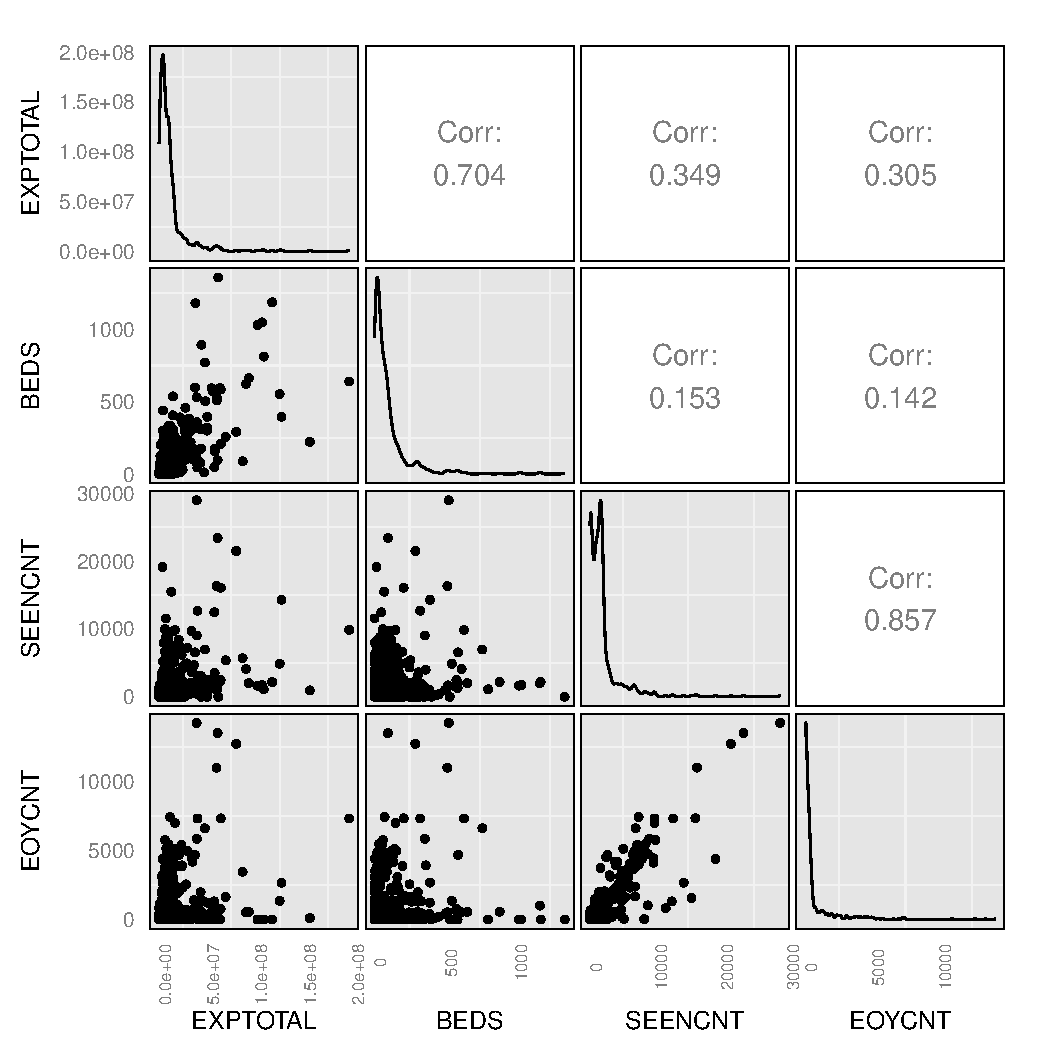
\includegraphics[width=\linewidth,height=8cm]{graphs/beamer-GREG_PlotMa-1} 

}



\end{knitrout}
}
\onslide*<3>{Fitting a linear model for \texttt{EXPTOTAL} with common slopes for \texttt{SEENCNT} and \texttt{EOYCNT} but a different slope for \texttt{BEDS} in each hospital type.
% latex table generated in R 3.2.2 by xtable 1.7-4 package
% Fri Jan 22 15:04:16 2016
\begin{table}[ht]
\centering
\caption{Model Summary} 
\begin{tabular}{rrrrr}
  \hline
 & Estimate & Std. Error & t value & Pr($>$$|$t$|$) \\ 
  \hline
(Intercept) & 1318589.11 & 912432.21 & 1.45 & 0.15 \\ 
  SEENCNT & 1033.94 & 310.63 & 3.33 & 0.00 \\ 
  EOYCNT & 2036.15 & 603.58 & 3.37 & 0.00 \\ 
  FINDIRCT2 & 78026.06 & 965237.62 & 0.08 & 0.94 \\ 
  hosp.type1:BEDS & 98139.28 & 3318.84 & 29.57 & 0.00 \\ 
  hosp.type2:BEDS & 39489.35 & 5644.51 & 7.00 & 0.00 \\ 
  hosp.type3:BEDS & 77578.37 & 15082.20 & 5.14 & 0.00 \\ 
  hosp.type5:BEDS & 36855.78 & 8650.48 & 4.26 & 0.00 \\ 
   \hline
\end{tabular}
\end{table}

}\onslide*<4>{
~\\[-1.25cm]





{\centering \animategraphics[width=\linewidth,height=8cm,controls,loop]{1}{graphs/beamer-GREG_PlotModelDiag_warningFALSE-}{1}{4}

}



}
\end{frame}

\begin{frame}[fragile]{Generalized Regression Estimator}
\begin{lrbox}{\mysavebox}
\begin{knitrout}\footnotesize
\definecolor{shadecolor}{rgb}{0.969, 0.969, 0.969}\color{fgcolor}\begin{kframe}
\begin{alltt}
\hlcom{#######################################}
\hlcom{### Select a pps to sqrt(BEDS) sample}
\hlcom{#######################################}
\hlkwd{library}\hlstd{(sampling)}   \hlcom{#load the 'sample' package }
                    \hlcom{#for the 'UPsystematic' function}
\hlstd{smho.} \hlkwb{<-}   \hlcom{# before sampling order the data set by hospital type}
  \hlstd{smho.[}\hlkwd{order}\hlstd{(smho.}\hlopt{$}\hlstd{hosp.type),]}

\hlstd{x} \hlkwb{<-} \hlstd{smho.[,}\hlstr{"BEDS"}\hlstd{]}
\hlstd{x[x} \hlopt{<=} \hlnum{5}\hlstd{]} \hlkwb{<-} \hlnum{5}      \hlcom{# recode small hospitals to have a minimum size}
\hlstd{x} \hlkwb{<-} \hlkwd{sqrt}\hlstd{(x)}

\hlstd{n} \hlkwb{<-} \hlnum{80}             \hlcom{#sample size}
\hlstd{IP}  \hlkwb{<-} \hlstd{n}\hlopt{*}\hlstd{x}\hlopt{/}\hlkwd{sum}\hlstd{(x)}

\hlkwd{set.seed}\hlstd{(}\hlnum{428274453}\hlstd{)}
\hlstd{sam} \hlkwb{<-} \hlkwd{UPsystematic}\hlstd{(IP)}

\hlstd{sam.dat} \hlkwb{<-} \hlstd{smho.[sam}\hlopt{==}\hlnum{1}\hlstd{, ]}
\hlstd{sam.dat}\hlopt{$}\hlstd{IP} \hlkwb{<-} \hlstd{IP[sam}\hlopt{==}\hlnum{1}\hlstd{]}   \hlcom{#the design weight}
\hlstd{sam.dat}\hlopt{$}\hlstd{d} \hlkwb{<-} \hlnum{1}\hlopt{/}\hlstd{IP[sam}\hlopt{==}\hlnum{1}\hlstd{]}   \hlcom{#the design weight}
\end{alltt}
\end{kframe}
\end{knitrout}
\end{lrbox}
\onslide*<1>{~\\[-1cm] We select a sample of hospitals with probability  proportional to the square root of \texttt{BEDS} using a systematic sample. 
 \usebox{\mysavebox}
}
\begin{lrbox}{\mysavebox}
\begin{knitrout}\footnotesize
\definecolor{shadecolor}{rgb}{0.969, 0.969, 0.969}\color{fgcolor}\begin{kframe}
\begin{alltt}
\hlkwd{library}\hlstd{(survey)} \hlcom{#load the 'survey' package }
\hlcom{#1. build a 'design' object}
\hlstd{sam.dsgn} \hlkwb{<-}
  \hlkwd{svydesign}\hlstd{(} \hlkwc{ids} \hlstd{=} \hlopt{~}\hlnum{1}         \hlcom{# no clusters}
            \hlstd{,}\hlkwc{data} \hlstd{= sam.dat}   \hlcom{# the sample data }
            \hlstd{,}\hlkwc{fpc} \hlstd{=} \hlopt{~}\hlstd{IP}        \hlcom{# incl. prob}
            \hlstd{,}\hlkwc{pps}\hlstd{=} \hlstr{"brewer"}\hlstd{)}    \hlcom{# variance approx. method}
 \hlcom{#the model we use for the GREG}
\hlstd{lmod2} \hlkwb{<-} \hlkwd{lm}\hlstd{(EXPTOTAL} \hlopt{~} \hlstd{SEENCNT} \hlopt{+} \hlstd{EOYCNT} \hlopt{+} \hlstd{hosp.type}\hlopt{:}\hlstd{BEDS,} \hlkwc{data}\hlstd{=smho.)}
\hlcom{#2. compute pop totals of auxiliaries}
\hlstd{pop.tots} \hlkwb{<-} \hlkwd{colSums}\hlstd{(}\hlkwd{model.matrix}\hlstd{(lmod2))} \hlcom{#Inefficient but convenient!}

\hlcom{#3. use 'calibrate' to compute the new weights}
\hlstd{sam.cal} \hlkwb{<-}
  \hlkwd{calibrate}\hlstd{(}\hlkwc{design} \hlstd{= sam.dsgn,}
            \hlkwc{formula} \hlstd{=} \hlopt{~} \hlstd{SEENCNT} \hlopt{+} \hlstd{EOYCNT} \hlopt{+} \hlstd{hosp.type}\hlopt{:}\hlstd{BEDS,}
            \hlkwc{population} \hlstd{= pop.tots,}
            \hlkwc{calfun}\hlstd{=}\hlstr{'linear'} \hlstd{)}
\end{alltt}
\end{kframe}
\end{knitrout}
\end{lrbox}
\onslide*<2>{ Now we use the \texttt{survey} package to calibrate the weights.
 \usebox{\mysavebox}
Setting argument \texttt{calfun='linear'} in \texttt{'calibrate'} results in the GREG weights, other calibration function are possible, already built-in are \texttt{'raking'} and \texttt{'logit'}. 
}
\begin{lrbox}{\mysavebox}
\begin{knitrout}\footnotesize
\definecolor{shadecolor}{rgb}{0.969, 0.969, 0.969}\color{fgcolor}\begin{kframe}
\begin{alltt}
\hlcom{#BEDS by hospital type}
\hlkwd{svyby}\hlstd{(}\hlopt{~}\hlstd{BEDS,} \hlkwc{by}\hlstd{=}\hlopt{~}\hlstd{hosp.type,} \hlkwc{design}\hlstd{=sam.cal,} \hlkwc{FUN}\hlstd{=svytotal)}
\end{alltt}
\begin{verbatim}
##   hosp.type  BEDS           se
## 1         1 37978 4.100694e-12
## 2         2 13066 1.122603e-12
## 3         3  9573 3.028628e-13
## 5         5 10077 7.135892e-13
\end{verbatim}
\begin{alltt}
\hlcom{#SEENCNT and EOYCNT}
\hlkwd{svytotal}\hlstd{(}\hlopt{~}\hlstd{SEENCNT}\hlopt{+}\hlstd{EOYCNT, sam.cal)}
\end{alltt}
\begin{verbatim}
##           total SE
## SEENCNT 1349241  0
## EOYCNT   505345  0
\end{verbatim}
\begin{alltt}
\hlstd{pop.tots}
\end{alltt}
\begin{verbatim}
##     (Intercept)         SEENCNT          EOYCNT hosp.type1:BEDS 
##             725         1349241          505345           37978 
## hosp.type2:BEDS hosp.type3:BEDS hosp.type5:BEDS 
##           13066            9573           10077
\end{verbatim}
\end{kframe}
\end{knitrout}
\end{lrbox}
\onslide*<3>{~\\[-0.9cm]
Now we check if the calibration constrains are satisfied:
\usebox{\mysavebox}
}

\end{frame}

\begin{frame}{Generalized Regression Estimator}
\begin{itemize}
  \item<1-> Nothing prevents the GREG weights from becoming negative, which is theoretically not a problem, as long as we infer to the population (or sub-populations) to which we calibrated. 
  \item<2-> However the effects might be catastrophic of domain estimation, in case of estimation domains that where not considered in the calibration. 
  \item<3-> In general, it is advisable to only use calibrated weights to infer to the whole population or sub-populations that are found in the marginal totals used for the calibration!
  \item<4> Design weights can always be used to do unbiased domain estimation, although the precision of these estimates can be very poor.
\end{itemize}
\end{frame}


\begin{frame}[fragile]{The Variance of the \\ Generalized Regression Estimator}
Calibrated weights are \textbf{not} independent of the selected sample, i.e. they are random variables.
Thus, the variance of the GREG estimator cannot be estimated as straightforwardly as for the $\pi$-estimator.
\onslide*<1>{
 We can write its approximate variance as
\begin{equation*}
 \AV{\hat{\tau}_\text{GREG}}  = \sum_{k \in \mathcal{U}} \sum_{l \in \mathcal{U}} \left( \pi_{kl} - \pi_k \pi_l \right)  \dfrac{E_k}{\pi_k} \dfrac{E_l}{\pi_l} \;{,}
 \end{equation*}
where $E_k = y_k - y_k^0$, $y_k^0= \mathbf{x}_x^\top \boldsymbol\beta $ and 
\begin{equation*}
 \boldsymbol\beta=\left( \underset{k \in \mathcal{U} }{\sum } c_k \mathbf{x}_{k} (\mathbf{x}_{k})^\top \right)^{-1} \underset{k \in \mathcal{U}}{\sum} c_k \mathbf{x}_{k} y_{k}\;{.}
\end{equation*}
}
\onslide*<2>{
A variance estimator for $\hat{\tau}_\text{GREG}$ is given by
 \begin{equation*}
 \Vest{\hat{\tau}_\text{GREG}}  = \sum_{k \in \mathfrc{s}} \sum_{l \in \mathfrc{s}} \dfrac{\left( \pi_{kl} - \pi_k \pi_l \right)}{\pi_{kl}} g_k \dfrac{e_k}{\pi_k} g_l \dfrac{e_l}{\pi_l} \;{,}
 \end{equation*}
where $e_k = y_k - \hat{y}_k$ and $\hat{y}_k = \mathbf{x}_x^\top \widehat{\boldsymbol\beta}$. 
}

\begin{lrbox}{\mysavebox}
\begin{knitrout}\footnotesize
\definecolor{shadecolor}{rgb}{0.969, 0.969, 0.969}\color{fgcolor}\begin{kframe}
\begin{alltt}
\hlkwd{svytotal}\hlstd{(}\hlopt{~}\hlstd{EXPTOTAL, sam.dsgn)}
\end{alltt}
\begin{verbatim}
##             total       SE
## EXPTOTAL 9.55e+09 7.72e+08
\end{verbatim}
\begin{alltt}
\hlkwd{svytotal}\hlstd{(}\hlopt{~}\hlstd{EXPTOTAL, sam.cal)}
\end{alltt}
\begin{verbatim}
##             total       SE
## EXPTOTAL 9.03e+09 5.92e+08
\end{verbatim}
\end{kframe}
\end{knitrout}
\end{lrbox}
\onslide*<3>{Compare the estimates for the total expenditure with calibrated and design weights.
\usebox{\mysavebox}
We find that $\hat{\tau}_\text{GREG} /  \hat{\tau}_\pi  = 1.0581$, but 
$ \Vest{\hat{\tau}_\text{GREG}} /  \Vest{\hat{\tau}_\pi}  = 1.7006$.
}


\end{frame}

\begin{frame}[allowframebreaks]\frametitle{Literature}
%\scriptsize
  \begin{thebibliography}{10}
   \setbeamertemplate{bibliography item}[book]
  \bibitem{LittleRubin2002}
  R.J.A.~Little, D.B.~Rubin.
    \newblock Statistical Analysis with Missing Data.
    \newblock {\em Wiley Interscience}, 1999.
   \setbeamertemplate{bibliography item}[book]
  \bibitem{SaerndalLundstroem2005}
  C.-E.~S\"{a}rndal, S.~Lundstr\"{o}m.
    \newblock Estimation in Surveys with Nonresponse.
    \newblock {\em Wiley}, 2005.
  \end{thebibliography}
  
\end{frame} 


% \begin{frame}{Two-phase Approach with a GLM}
%  
%  
% \end{frame}
 
 %System time of variance calculation
 
 %Variance of the GREG
 
 %Taylor linearization of a ratio estimatir V(x/y)\neq V(x)/V(y) not even E(x/y) \neq E(x)/E(y) is close enought!
 %Influence Funktions
 
 %Resampling Methods

%Ratio estimator  Saerndal2005 42

\end{document}
